% ----------------------------------------------------------
% Proposta
% ----------------------------------------------------------
\chapter{Proposta de projeto: \fancyname}
\label{chp:proposta}

A presente proposta tem como objetivo principal coletar memória de recursos computacionais virtuais de modo a conseguir: 
(1) identificar a fonte da evidência, mesmo se o recurso virtual não existir mais; 
(2) descrever o sistema antes e depois do incidente;
(3) transportar e armazenar a memória coletada de uma forma que garanta sua integridade e confidencialidade; e
(4) não violar a jurisdição e a privacidade de outros usuários que porventura tenham recursos alocados no mesmo servidor físico.
%
A solução aqui apresentada, denominada \fancyname, é descrita em detalhes a seguir.

\section{Descrição}
\label{sec:proposta-desc}

Em sistemas computacionais executados sobre uma infraestrutura física (i.e., não virtualizada), pode-se fazer uma associação direta entre um recurso qualquer, como uma informação da memória, imagem de disco ou pacotes trafegando na rede, e sua origem correspondente.
%
Já em sistemas construídos sobre uma infraestrutura virtual, em especial quando esta é auto-escalável, os recursos computacionais são altamente voláteis e, portanto, podem ser desalocados a qualquer momento.
%
Para conseguir correlacionar uma evidência a sua origem volátil, é necessário utilizar outro elemento em que persista a relação fonte-evidência, o que na presente proposta é feito por meio de contêineres linux (LXC).
%
Embora um contêiner seja um \textit{software} e, portanto, também volátil, cada imagem compilada e sua execução na forma de contêiner são normalmente atrelados a um \textit{hash} que identifica univocamente essa relação.
%
O contêiner também permite identificar com mais precisão a fonte de uma evidência, uma vez que é possível dividir as partes de um sistema em contêineres: por exemplo, um contêiner para o motor de páginas dinâmicas (e.g., Apache%\cite{Tomcat}
), outro com a lógica de negócios (e.g., \textit{golang}%\cite{Google}
) e um terceiro para um banco de dados (e.g., \textit{Cassandra}%\cite{Cassandra}
).

%\marcosT{O parágrafo estava muito grande, então quebrei aqui. O problema é que falta uma frase para ligar a frase a seguir ao contexto da discussão... Coloque uma frase aqui, deixando claro qual requisito você quer satisfazer com essa ideia de ``interromper temporariamente a execução do contêiner''. Aplique isso para TUDO que for proposta: o leitor tem que saber de antemão pra que você está fazendo alguma coisa, ou vai ficar se perguntando ``Espera, mas pra que fazer isso?!'' - Hamilton: Feito}
A cópia de memória não é uma atividade atômica, pois ela é executada em conjunto com outros processos. 
%
Portanto, caso um desses processos seja um código malicioso apagando traços de sua existência da memória do contêiner, informações possivelmente importantes para a investigação podem acabar sendo perdidas. 
%
Com o objetivo de deixar o processo de cópia da memória mais atômico, \fancyname interrompe temporariamente a execução do contêiner, realiza a cópia de sua memória, e em seguida retoma sua execução. 
%
Essa técnica, que é semelhante àquela adotada em \cite{RafiqueStaticLiveDigitalForensics:2013} para VMs, produz um instantâneo da memória volátil do contêiner; isso permite sua análise em um estado de repouso, ou seja, sem a necessidade de ter o contêiner em execução.
%
Ao realizar a coleta em intervalos de tempo adequados, é possível construir um histórico do estado da memória durante a execução no contêiner.
%
%\marcosT{A ligação entre as frases anterior e a seguir está bem ruim... você parece estar mudando completamente de assunto... Acredito que faltou uma frase dizendo que ``''salvar toda a memória'' pode se tornar um problema, reforçar isso com as duas frases que já estão a seguir, e depois dizer que você vai resolver.}

A maioria das técnicas forenses mais usadas atualmente são voltadas à obtenção da informação em sua totalidade, seja via cópia bit a bit, seja por meio da obtenção do \textit{hardware} físico \cite{SimouCloudChlng:2014} \cite{BemPastPresentFuture:2008}. 
%
Embora tais técnicas possam parecer interessantes à primeira vista, elas muitas vezes acabam sendo responsáveis por um problema: o crescente volume de informações que os investigadores precisam analisar \cite{QuickIncreaseVolumeImpact:2014}.
%
Para mitigar essa dificuldade, em \fancyname são adotadas duas estratégias: a primeira é a definição de um volume de dados que possa ser considerado \textit{suficiente} para a realização de uma investigação; a segunda é a definição de uma \textit{idade máxima} para a evidência enquanto o sistema trabalha em condições normais, isto é, quando não está sob ataque.
%
Para detectar e analisar intrusões na memória de processos, é necessário ter uma cópia da memória antes e depois da intrusão \cite{CaseMemoryForensics:2014}. 
%
Assim, a solução proposta implementa uma janela de instantâneos de memória cobrindo um intervalo de tempo pré-definido, como ilustrado na Fig. \ref{fig:janela}. 
%
Em condições normais de operação, as evidências são coletadas com certa periodicidade e coletas que atingem uma determinada idade são descartadas.
%
Em contraste, após a detecção de um evento de ataque (e.g., por um sistema de detecção de intrusões), \fancyname deixa de descartar as coletas mais antigas do \textit{log} de monitoramento, sendo possível conhecer o sistema antes e depois do ataque e, assim, avaliar sua evolução.
%
%\marcosR{Não sei por que você está utilizando $\backslash\backslash$ no final das suas frases, mas pare de fazer isso... deixe o LaTeX se virar com a formatação. No final, quando você tiver tudo escrito, aí pode fazer algum sentido se preocupar com formatação, mas não antes disso... - Hamilton: é pra formatação mesmo :-) OK vou deixar o latex se virar}
%

\begin{figure}[htb!]
\footnotesize
\caption{Janela deslizante de coleta de evidência}
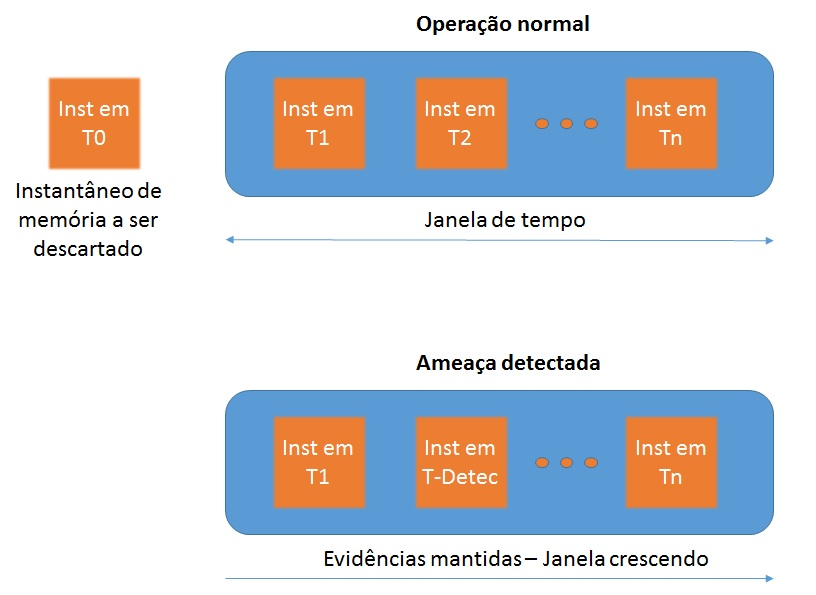
\includegraphics[scale=0.40]{janela.jpg}
\centering
\label{fig:janela}
\begin{center}
Fonte: Próprio autor 
\end{center}
\end{figure}

%\marcosT{Essa frase não faz sentido: não se ``assina'' nada com um ``hash''. Você pode ``calcular o hash'' ou ``assinar um dado'' (e.g., um dado juntamente com o hash de alguma coisa). Revise essa frase... - Hamilton: Feito}
Para persistir a relação evidência-origem e garantir a integridade da mesma, a presente proposta calcula o hash do par [evidência, identificador da imagem do contêiner] e armazena a tripla [hash, identificador da imagem do contêiner, evidência].
%
Para evitar eventuais problemas com o armazenamento desses dados em países com jurisdições diferentes daquelas que devem ser aplicadas na investigação em questão, as evidências coletadas são armazenadas em um local físico fora da nuvem, após serem transportadas por meio de um canal seguro (e.g., via TLS ( \textit{Transport Layer Security} -- Camada de Transporte Seguro ) \cite{DierksT2008}).
%

\section{Implementação}
\label{sec:proposta-impl}

%\marcosT{CLAREZA: quais ataques? Onde estão esses objetivos (diga a seção!!!)? Perceba que não tem qualquer seção com esse nome: você espera realmente que o leitor procure no seu texto onde eles estão...? - Hamilton: Feito}

\begin{figure}[htb!]
\footnotesize
\caption{Arquitetura geral da solução Dizang}
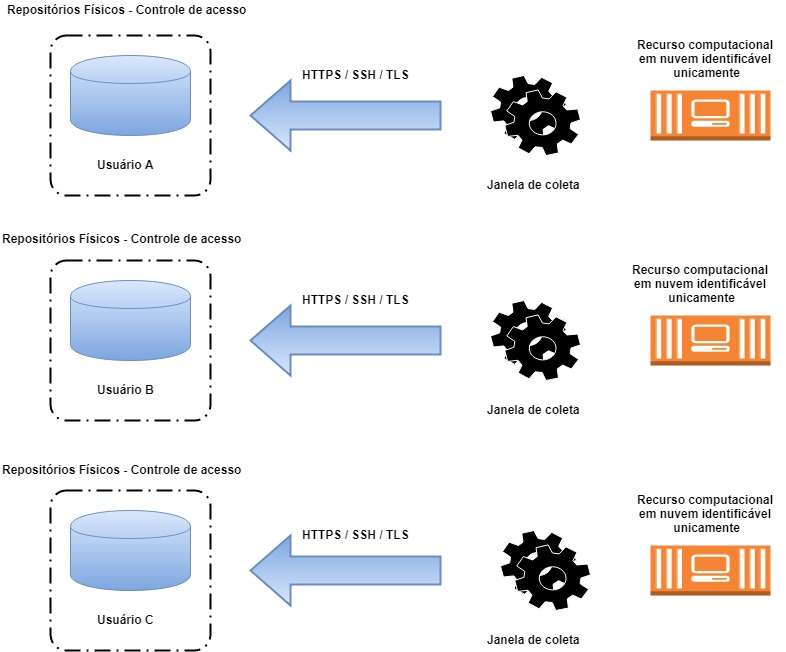
\includegraphics[scale=0.41]{solucao.jpg}
\centering
\label{fig:Solucao}
\begin{center}
Fonte: Próprio autor 
\end{center}
\end{figure}


Os métodos propostos foram implementados em uma plataforma de testes visando avaliar a eficácia de \fancyname em coletar as informações de memória dos contêineres de forma reprodutível, sem violar jurisdições ou a privacidade de usuários.
%
A solução, ilustrada na Fig. \ref{fig:Solucao}, consistiu na criação de 1 VM  ( \textit{Virtual Machine} -- Máquina Virtual ) usando o Oracle Virtual Box 5.0 \cite{VirtualBox} 
em um notebook Intel i5 de 2.30Mhz e 4Gb de RAM com sistema operacional de 64 bits.
%
Essas VMs possuem 2 Gb de memória RAM e emulam apenas 1 processador, e em cada uma delas foi instalado o Docker Engine 1.10%\cite{DockerInc} 
e a API Docker 1.21%\cite{DockerInc}
, com os quais foram criados 3 contêineres executando o nginx 1.0%\cite{nginx}
 em diferentes portas. 
%
Usando uma aplicação Java que descobre o identificador de processo associado a cada contêiner, pode-se copiar conteúdo do \textit{descritor de alocação de memória não uniforme} (\textbf{/proc/pid/numa\_maps}), o qual contém a alocação das páginas de memória, os nós que estão associados a essas páginas, o que está alocado e suas respectivas políticas de acesso \cite{UnixManPagesNumaMaps}.
%
A cópia e gravação do arquivo é tal que, a cada minuto, a aplicação (1) pausa o contêiner em questão, (2) copia a diretório \textbf{numa\_maps}, (3)  concatena os dados obtidos com o \textit{hash} de identificação da imagem do contêiner, (4) calcula o \textit{hash} do conjunto e (5) salva o resultado em um arquivo cujo nome é o identificador da imagem do contêiner e a extensão é \textbf{.mem}. 
%
Após a conclusão do processo de cópia, a mesma aplicação verifica se existem arquivos \textbf{.mem} em disco mais antigos que um certo intervalo de tempo ``t'', descartando-os.
%

%\marcosT{IMPORTANTE: discuta em alguns parágrafos os resultados. Até aqui, você só disse o que fez, mas não falou nada sobre o que isso traz de impactos positivos ou negativos. Por exemplo: quanto tempo demora a cópia (isso pode ser crítico para um processo que opera em tempo real, já que ele será pausado...)? Enfim, tire conclusões dos experimentos, porque senão os experimentos não têm qualquer utilidade para o leitor... Quanto mais completa a discussão (não só ``tempos'', mas também memória, quantidade de dados gerados por hora, uso de banda, etc.), melhor. Gráficos e tabelas com dados obtidos são muito bem vindos. - Hamilton: Feito}

%\marcosT{IMPORTANTE: Discuta também a relação entre o que foi feito e os ataques de injeção mencionados na introdução. O seu texto inicialmente menciona tais ataques como parte do seu foco, mas nunca mais retoma a existência deles depois que você descreve a solução... Não precisa ser uma discussão longa, mas ao menos algumas considerações sobre o porquê de você conseguir analisar tais ataques usando a técnica proposta - Hamilton: Feito.}
%

\section{Resultados experimentais}
\label{sec:proposta-exp}

Para avaliar a efetividade de \fancyname na coleta de evidências, alguns experimentos foram realizados usando o ambiente implementado (descrito na Seção \ref{sec:proposta-impl}).
%
Primeiramente, o sistema foi configurado para realizar coletas de memória em intervalos de 1 minuto, salvá-las em disco externo e apagar amostras coletadas há mais de 5 minutos. 
%
O sistema foi então executado por 30 minutos, tempo durante o qual foram coletadas como métricas (1) o uso de espaço em disco utilizado pelos instantâneos de memória salvos e (2) o tempo de pausa no contêiner necessário para a cópia delas.
%
A cada coleta, foi executado o comando \texttt{du -sh *.mem} do \textit{Unix} no disco de armazenamento externo, para retornar a lista dos arquivos onde os instantâneos de memória foram armazenados e o espaço em disco ocupado pelos mesmos. 
%
Ao fim do experimento, os contêineres foram removidos.


A ocupação em disco devido aos instantâneos de memória capturados durante o experimento é mostrada no gráfico da Fig. \ref{fig:evolucao-coleta}. 
%
O gráfico mostra que o aumento do uso do espaço em disco é linear e o crescimento se interrompe quando é atingido o limite de tempo configurado para a janela, pois as coletas com tempo de vida maior que tal limite são apagadas do disco. 
%
Assim, que a solução mantém sob controle o espaço em disco ocupado pelas amostras coletadas.
%
Ao mesmo tempo, instantâneos de memória salvos pela solução depois que os contêineres são removidos continuam no disco da máquina, podendo ser associados a sua origem (i.e., contêiner e imagem), conforme esperado para uma análise forense.
%
Essa capacidade se mantém após a detecção de uma ameaça, pois nesse caso coletas mais antigas deixam de ser apagadas.
%
Logo, é possível descrever o estado do sistema antes e depois do incidente \cite{CaseMemoryForensics:2014}, permitindo-se, por exemplo, que ataques de injeção de código em memória sejam analisados.


%\marcos{EVITE REDUNDÂNCIA ENTRE GRÁFICO E TABELA. Faz sentido apenas se um deles for trazer informações adicionais (e, nesses casos, em geral o gráfico/tabela acaba tendo algum highlight, para deixar a utilidade dessa redundância)
%\begin{table}[htb!]
%\centering
%\caption{Evolução do uso do espaço em disco}
%\label{tab:results-size}
%\begin{tabular}{c|c}
%\hline
%Tamanho total ocupado (KBytes) & Tempo (segundos) \\ \hline
%240                            & 1                \\ \hline
%480                            & 2                \\ \hline
%720                            & 3                \\ \hline
%960                            & 4                \\ \hline
%1200                           & 5                \\ \hline
%1200                           & 6                \\ \hline
%1200                           & 7                \\ \hline
%1200                           & 8                \\ \hline
%1200                           & 9                \\ \hline
%1200                           & 10                \\ \hline
%1200                           & 11                \\ \hline
%1200                           & 12                \\ \hline
%1200                           & 13                \\ \hline
%1200                           & 14                \\ \hline
%1200                           & 15                \\ \hline
%1200                           & 16                \\ \hline
%1200                           & 17                \\ \hline
%1200                           & 18                \\ \hline
%1200                           & 19                \\ \hline
%1200                           & 20                \\ \hline
%1200                           & 21                \\ \hline
%1200                           & 22                \\ \hline
%1200                           & 23                \\ \hline
%1200                           & 24                \\ \hline
%1200                           & 25                \\ \hline
%1200                           & 26                \\ \hline
%1200                           & 27                \\ \hline
%1200                           & 28                \\ \hline
%1200                           & 29                \\ \hline
%1200                           & 30                \\ \hline
%\end{tabular}
%\end{table}

\begin{figure}[htb!]
\footnotesize
\caption{Evolução do uso do espaço em disco com o Dizang}
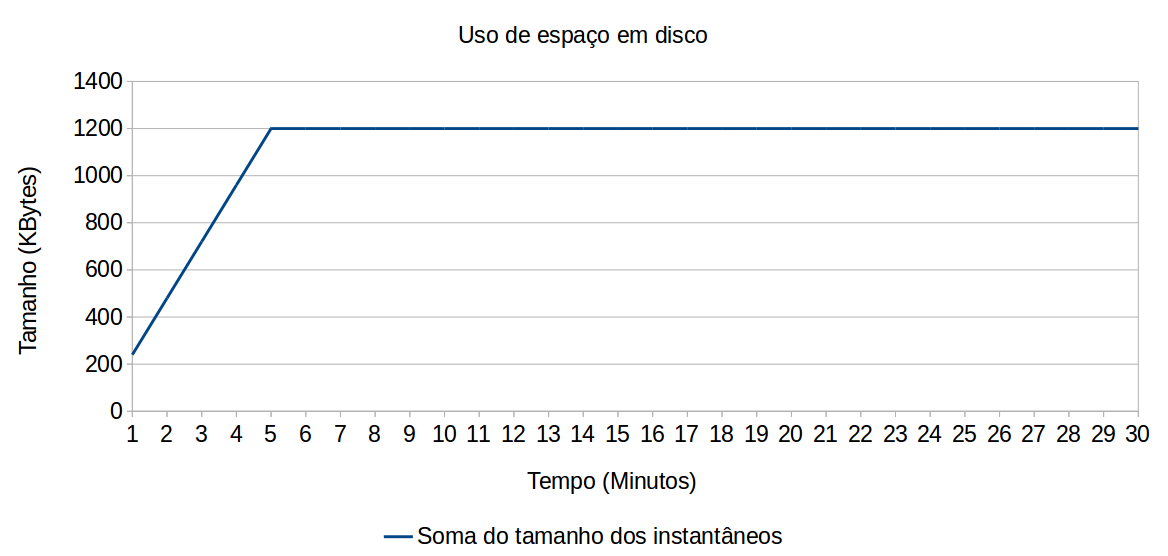
\includegraphics[scale=0.32]{evolucao-coleta.jpg}
\centering
\label{fig:evolucao-coleta}
\begin{center}
Fonte: Próprio autor 
\end{center}
\end{figure}


\begin{comment}
A Fig. \ref{fig:memoria_salva}, por sua vez, mostra uma listagem de alguns dos instantâneos de memória salvos pela solução depois que os contêineres são removidos. 
%
Nela pode-se ver que as coletas continuaram no disco da máquina mesmo após a remoção dos contêineres. 
%
Usando o identificador do contêiner e da imagem, consegue-se associar a evidência a sua origem (i.e., a imagem e o contêiner), conforme esperado para uma análise forense.
%
Essa capacidade se mantém após a detecção de uma ameaça, pois nesse caso coletas mais antigas deixam de ser apagadas.
%
Assim, é possível descrever o estado do sistema antes e depois do incidente \cite{Case_Memory_Forensics:2014}, permitindo-se, por exemplo, que ataques de injeção de código em memória sejam analisados.


\begin{figure*}[htb!]
\footnotesize
\caption{Exemplo de lista de instantâneos de memória.}
\fbox{
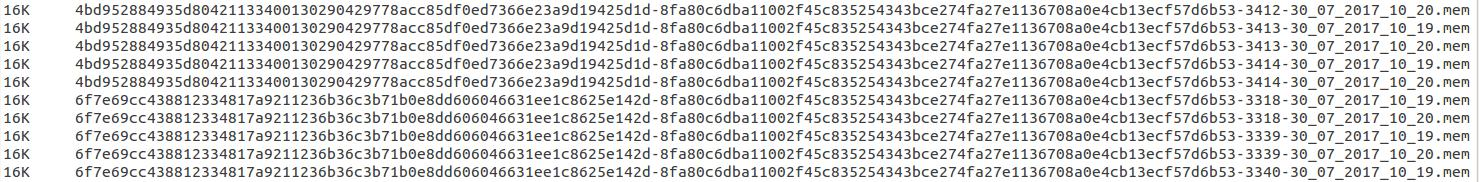
\includegraphics[scale=0.30]{memoria_salva.jpg}
}
\centering
\label{fig:memoria_salva}
\end{figure*}

\end{comment}

%No evento da detecção de uma ameaça a presente proposta deixa de apagar as coletas mais antigas. 
%
%Desta forma é capaz de descrever a história das alterações da memória do contêiner e com isso viabilizar a análise forense em busca das 4 vulnerabilidades de injeção de código em memória citadas no início do artigo. \marcos{Link bem fraco com introdução... pra que explicar em *detalhes* as vulnerabilidades na Introdução se você vai fazer uma explicação *superficial* de como elas são abordadas... Coloquei en passant para não dar a impressão de que você quis chamar a atenção para aquelas vulnerabilidades (sim, eu tinha pedido para você fazer esse link, mas um link tão fraco joga CONTRA você, não a favor...)}
%
%A viabilidade se dá pois consegue descrever o estado do sistema antes e depois do incidente \cite{Case_Memory_Forensics:2014}.
%

Uma potencial limitação da solução proposta é que a pausa de um contêiner para coleta de dados poder, em princípio, causar perdas no desempenho da aplicação sendo executada. 
%
Para avaliar esse impacto, durante o experimento foram medidos os tempos de cópia da memória do contêiner.
%
Os resultados são mostrados no gráfico da Fig. \ref{fig:memoria-copia}.
%
É possível notar que, após a inicialização da aplicação, o tempo para realizar a cópia é bastante reduzido, variando entre 20 e 40 milissegundos. 
%
Em especial, para contêineres executando um motor de páginas web dinâmicas, como é o caso do experimento em questão, essa latência deve ser pouco perceptível por usuários finais.


%\marcosT{Essas duas frases não é resultado do experimento, mas apenas característica da sua solução, então não faz muito sentido colocar aqui. Melhor mover essas considerações para o local em que você descreve essas características, fazendo merge com o texto que já esteja lá. Se você já fez essa discussão naquele ponto, então não precisa repetir. Se for fazer o merge, lembre-se (repita 2x ao dia, como um mantra): NÃO USE PRIMEIRA PESSOA EM TEXTOS FORMAIS EM PORTUGUÊS. - Hamilton: Feito. Desulpas, fraquejei :p}
%

%\begin{table}[htb!]
%\centering
%\caption{Tempo de cópia da memória de um contêiner}
%\label{tab:results-conteiner}
%\begin{tabular}{c|c}
%\hline
%Tempo de cópia (Milisegundos) & Coleta           \\ \hline
%149                           & 1                \\ \hline
%59                            & 2                \\ \hline
%23                            & 3                \\ \hline
%32                            & 4                \\ \hline
%35                            & 5                \\ \hline
%21                            & 6                \\ \hline
%17                            & 7                \\ \hline
%38                            & 8                \\ \hline
%16                            & 9                \\ \hline
%33                            & 10               \\ \hline
%17                            & 11               \\ \hline
%36                            & 12               \\ \hline
%18                            & 13               \\ \hline
%25                            & 14               \\ \hline
%31                            & 15               \\ \hline
%14                            & 16               \\ \hline
%33                            & 17               \\ \hline
%19                            & 18               \\ \hline
%13                            & 19               \\ \hline
%20                            & 20               \\ \hline
%18                            & 21               \\ \hline
%24                            & 22               \\ \hline
%8                             & 23               \\ \hline
%9                             & 24               \\ \hline
%19                            & 25               \\ \hline
%7                             & 26               \\ \hline
%8                             & 27               \\ \hline
%11                            & 28               \\ \hline
%35                            & 29               \\ \hline
%13                            & 30               \\ \hline
%\end{tabular}
%\end{table}

\begin{figure}[htb!]
\footnotesize
\caption{Tempo de cópia da memória de um contêiner}
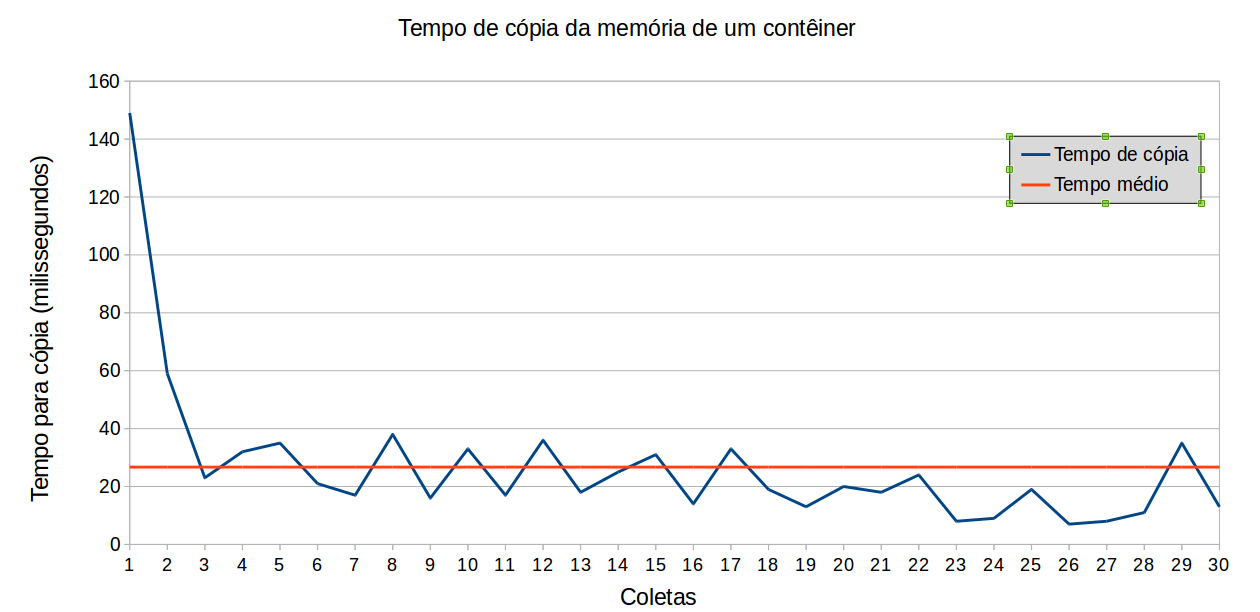
\includegraphics[scale=0.30]{memoria-copia.jpg}
\centering
\label{fig:memoria-copia}
\begin{center}
Fonte: Próprio autor 
\end{center}
\end{figure}

\section{Limitações}
\label{sec:proposta-limit}

Como a solução descrita tem como foco coletar informações de memória no espaço do usuário (\textit{user space}), ela não consegue acessar o espaço de kernel (\textit{kernel space}). 
%
Assim, \fancyname em princípio não provê suporte a técnicas de investigação de malware que se baseiam em informações do \textit{kernel space}, como, por exemplo, a comparação de informações do PEB ( \textit{Process Environment Block} -- Bloco para o Ambiente dos Processos ), que ficam no \textit{user space}, com informações do VAD ( \textit{Virtual Address Descriptor} -- Descritor de Endereços de Memória Virtual ), que fica no \textit{kernel space}. 
%
Análise de ameaças do tipo DKOM ( \textit{Direct Kernel Object Manipulation} -- Manipulação Direta dos Objetos do Kernel ) também não se beneficiam com a solução aqui proposta. 
%\marcosT{Não entendi a ``associação com o contêiner'' aqui. Você quer dizer que ``não se beneficiam com a solução aqui proposta'' ou outra coisa? Você não definiu o que seria a tal ``associação com o contêiner'' fora do contexto da sua solução, então ficou confuso - Hamilton: Feito}.


\section{Conclusões e trabalhos futuros}
\label{sec:proposta-concl}

%\marcosT{Uma boa conclusão retoma, logo na primeira frase, o problema que ela se propunha a resolver. Comece com uma ou mais frases nesse sentido, (nota: \textbf{sem} copiar+colar de outro ponto do texto). - Hamilton: Feito} \marcosT{Só que não: eu disse para você retomar o \textbf{problema} na sua primeira frase. Sua frase começa retomando a \textbf{solução}. Essa que você colocou como primeira seria boa como uma segunda frase, em que você reforça como resolve o problema - Hamilton: Acho que agora foi :)}
%
Ameaças digitais que atuam diretamente na memória de sistema não costumam deixar rastros em disco após terem os recursos correspondentes desalocados, dificultando análises forenses posteriores.
%
Esse problema é especialmente notável em sistemas de computação em nuvem, nos quais a alocação e desalocação de recursos virtualizados (e.g., VMs e contêineres) é frequente.
%
Essa característica, aliada a aspectos como multi-inquilinato e multi-jurisdição de nuvens computacionais, dificulta a coleta de evidências para a investigação de incidentes.


Nesse cenário, a proposta apresentada visa relacionar o instantâneo de memória a sua origem, utilizando o \textit{hash} calculado da imagem do contêiner como identificador da evidência armazenada.
%
Para evitar uso excessivo de memória, a quantidade de dados armazenados usa uma janela de armazenamento, o que permite descrever a memória antes e depois de um ataque (e.g., de injeção de memória). 
%
Combinada com uma ferramenta para identificação de ameaças, essas características de \fancyname o transformam em uma solução poderosa para prover evidências e, assim, viabilizar análises forenses na nuvem.
%
%Cabe notar, entretanto, que muitas ferramentas de análise malware disponíveis no mercado necessitam que todo o conteúdo da memória da máquina esteja disponível para realização da análise (e.g., FROST \cite{Dykstra_FROST:2013} e Volatility Framework \cite{VolatilityFoundation2014}), o que inviabiliza seu uso diretamente sobre a memória de processos conforme coletado por \fancyname.
%
%Portanto, como trabalho futuro, pretende-se desenvolver uma ferramenta de detecção de ameaças mais flexível, que, embora potencialmente utilize técnicas similares àquelas adotadas em sistemas atuais, seja capaz de fazê-lo sem necessariamente ter acesso à memória completa da máquina.
%

Como trabalho futuro, pretende-se estudar o impacto provocado pela pausa do contêiner no desempenho de um sistema em produção e realizar uma análise da memória dos contêineres deste mesmo sistema utilizando as coletas feitas por \fancyname. 
%
Com esses resultados pretende-se implementar uma ferramenta mais flexível, que não precise ter acesso a memória completa da máquina, requisito comum de ferramentas de análise de malware atuais (e.g., FROST \cite{DykstraFROST:2013} e Volatility Framework \cite{VolatilityFoundation2014}).


\section{O que foi feito e cronograma esperado para os próximos passos}
\label{sec:proposta-prox}

A presente proposta está planejada para ser executada em 3 fases.
%
A primeira fase tem por objetivo encontrar uma forma de relacionar a evidência coletada de um contêiner a sua origem de forma que o processo seja reprodutível. 
%
Para atingir este objetivo será implementado um protótipo de coleta de memória de uma máquina virtual executando contêineres em um notebook.
%
A segunda fase tem por objetivo encontrar uma forma de transportar a evidência coletada a um local de armazenamento garantindo a cadeia de custódia.
%
Para atingir este objetivo, será definida uma cadeia de custódia. De posse desta será realizada em uma nuvem computacional e envolverá o transporte da evidência para uma máquina física fora da nuvem.
%
A terceira parte tem por objetivo a realização da análise de alguma vulnerabilidade utilizando-se do material coletado na primeira fase do projeto.
%
As ações para se atingir este objetivo serão realizadas em um notebook com ferramental voltado a análise forense em memória.
%
Até então foram realizados com sucesso a duas primeiras partes do projeto.

%
Parte 1: A associação da evidência de memória coletada do contêiner de uma máquina virtual foi associada a sua origem através do \textit{hash} de identificação da imagem do contêiner. O processo de coleta foi reproduzido com sucesso diversas vezes.
%

Parte 2: O transporte da evidência para uma máquina física fora da nuvem utilizando camada de transporte seguro a assinatura da mensagem.
%

Para o restante do projeto, que consiste da parte 3, espera-se seguir o cronograma descrito na figura \ref{fig:cronograma} onde serão executadas as seguintes atividades.

\begin{itemize}
 \item \textbf{Estudo das ferramentas de análise de memória}: Onde serão avaliadas ferramentas de análise de memória na busca por alguma que consiga decodificar as informações coletadas 
 \item \textbf{Implementação / seleção de uma ferramenta de análise}: Nesta atividade será selecionada uma das ferramentas estudadas na atividade anterior. Caso nenhuma se mostre adequada, será implementada uma ferramente para o propósito da fase 3
 \item \textbf{Realização de análises com a ferramenta escolhida / criada}: Nesta fase ocorrerá a tentativa de analisar um malware encontrado em alguma coleta realizada na fase 1
\end{itemize}

\begin{figure}[htb!]
\footnotesize
\caption{Cronograma de projeto}
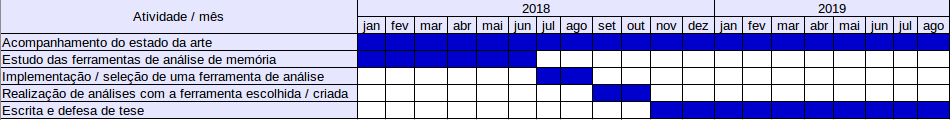
\includegraphics[scale=0.50]{crono-image.png}
\centering
\label{fig:cronograma}
\begin{center}
Fonte: Próprio autor 
\end{center}
\end{figure}

\section{Contribuições}
\label{sec:proposta-contrib}

A contribuição esperada da presente proposta é o de demonstrar que é possível coletar evidências de uma infraestrutura em nuvem de modo a atender os pré-requisitos de não violação de privacidade, não violação da jurisdição, reprodutibilidade do processo de coleta da evidência e garantia da cadeia de custódia.
%
Demonstrar que é possível realizar a análise de evidência de memória com apenas a parte \textit{user space} da memória coletada

